\section{系统运行}

\subsection{用户模块}

登陆模块包括用户的注册、登陆、找回密码、邮箱验证等功能。

\begin{figure}[thbp!]
	\centering
	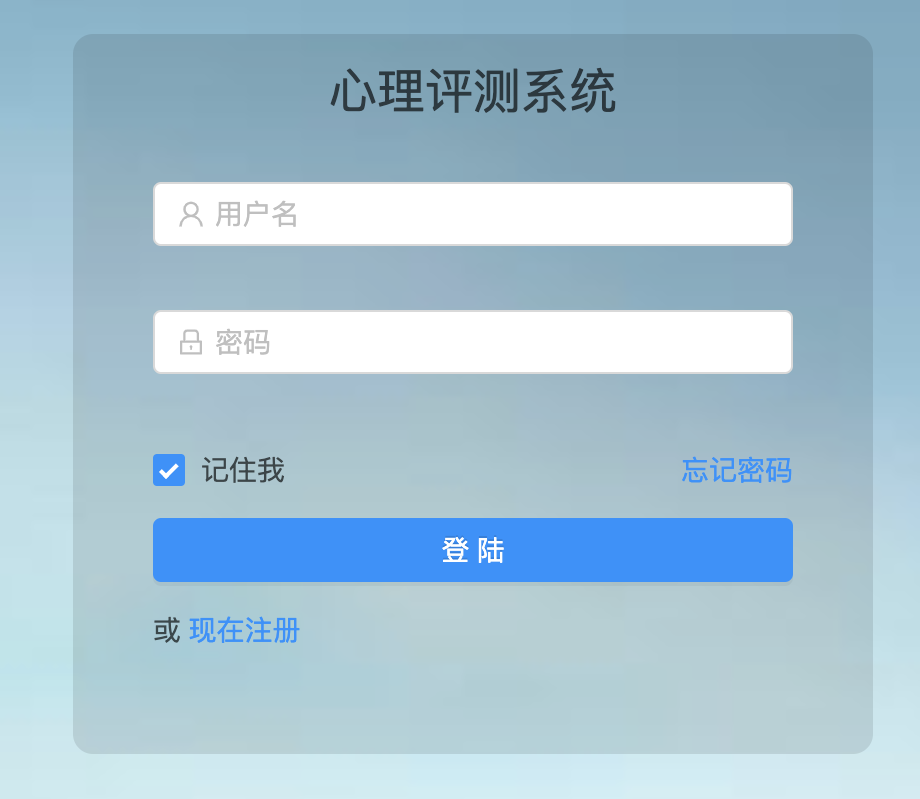
\includegraphics[width=0.7\linewidth]{figure/login}
	\caption{登陆界面}
	\label{fig:login}
\end{figure}

登陆界面的记住我可以设置浏览器中的cookie的过期时间为7天。

\begin{figure}[thbp!]
	\centering
	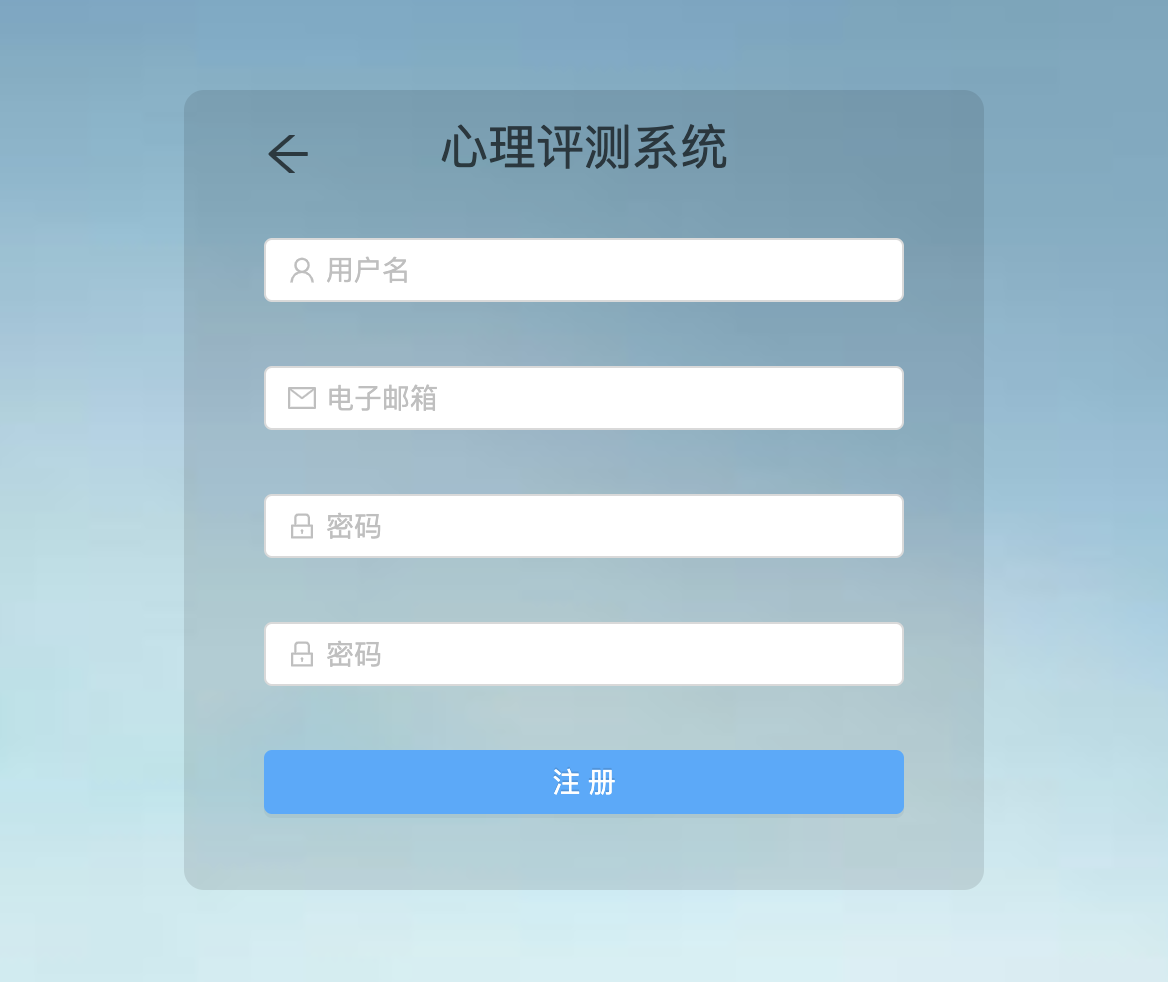
\includegraphics[width=0.7\linewidth]{figure/register}
	\caption{注册界面}
	\label{fig:register}
\end{figure}

\begin{figure}[thbp!]
	\centering
	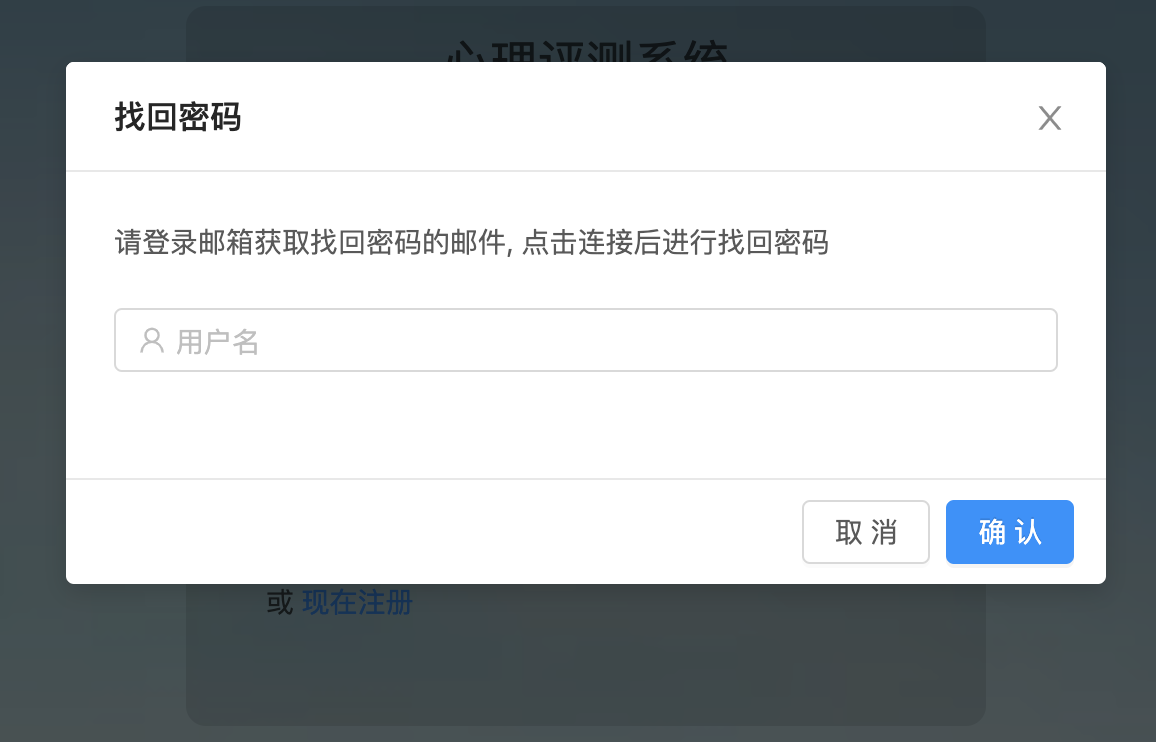
\includegraphics[width=0.6\linewidth]{figure/find_password}
	\caption{找回密码}
	\label{fig:find_password}
\end{figure}

\begin{figure}[thbp!]
	\centering
	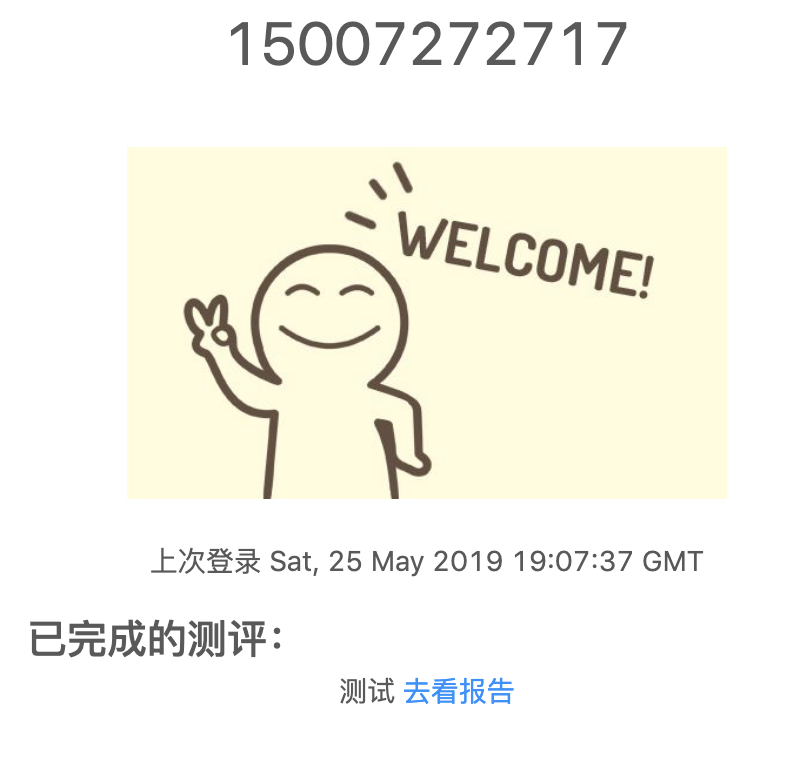
\includegraphics[width=0.6\linewidth]{figure/main}
	\caption{个人中心}
	\label{fig:main}
\end{figure}

\subsection{管理中心}

管理中心是管理员对试卷、用户、成绩进行筛选的模块。

\begin{figure}[thbp!]
	\centering
	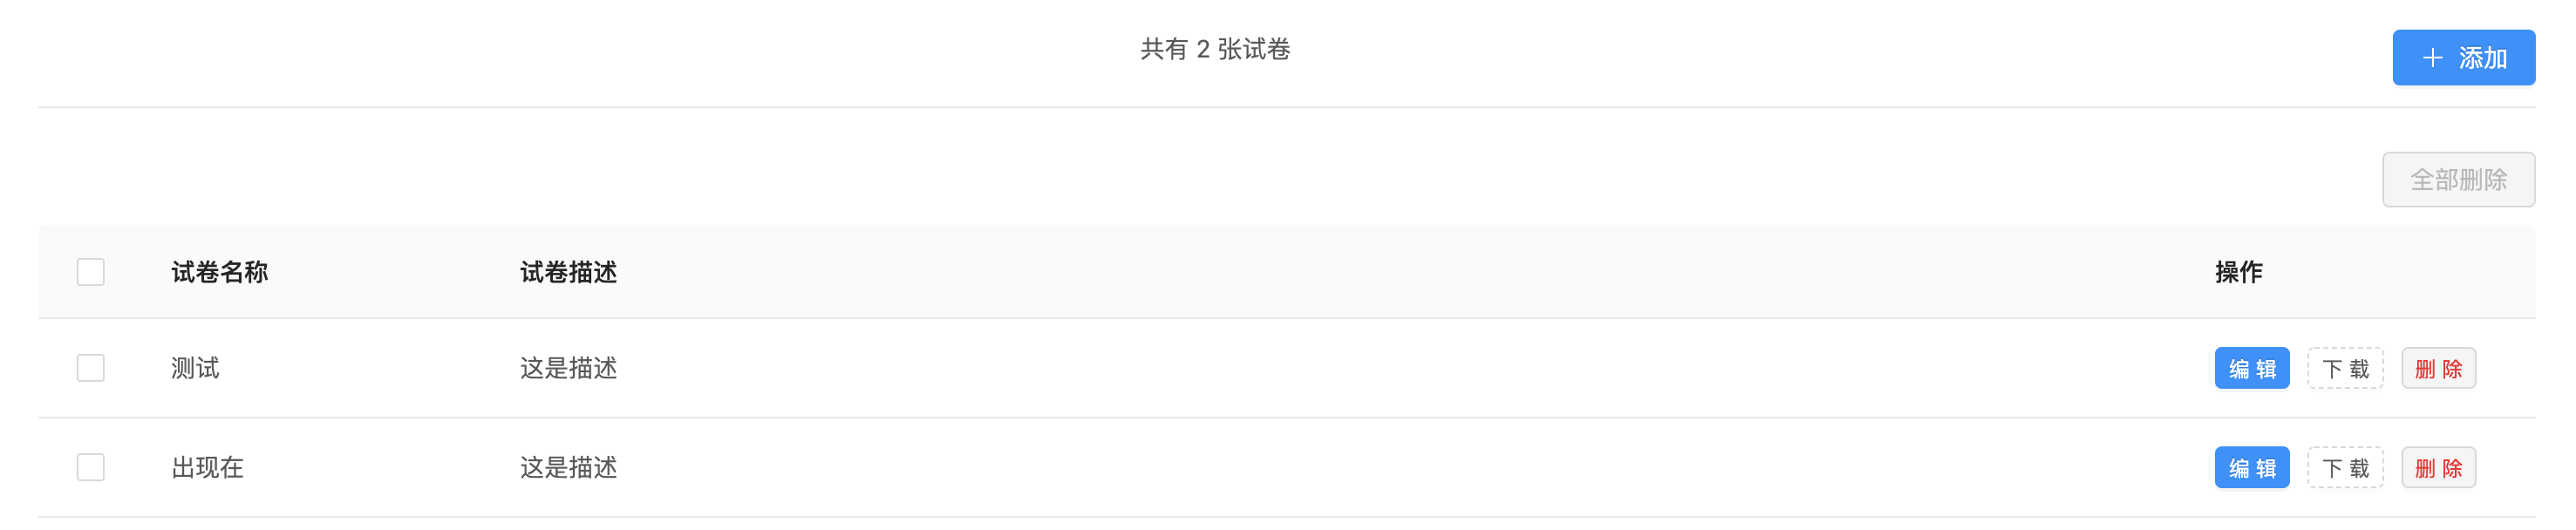
\includegraphics[width=1.0\linewidth]{figure/admin_paper}
	\caption{管理试卷}
	\label{fig:admin_paper}
\end{figure}

\begin{figure}[thbp!]
	\centering
	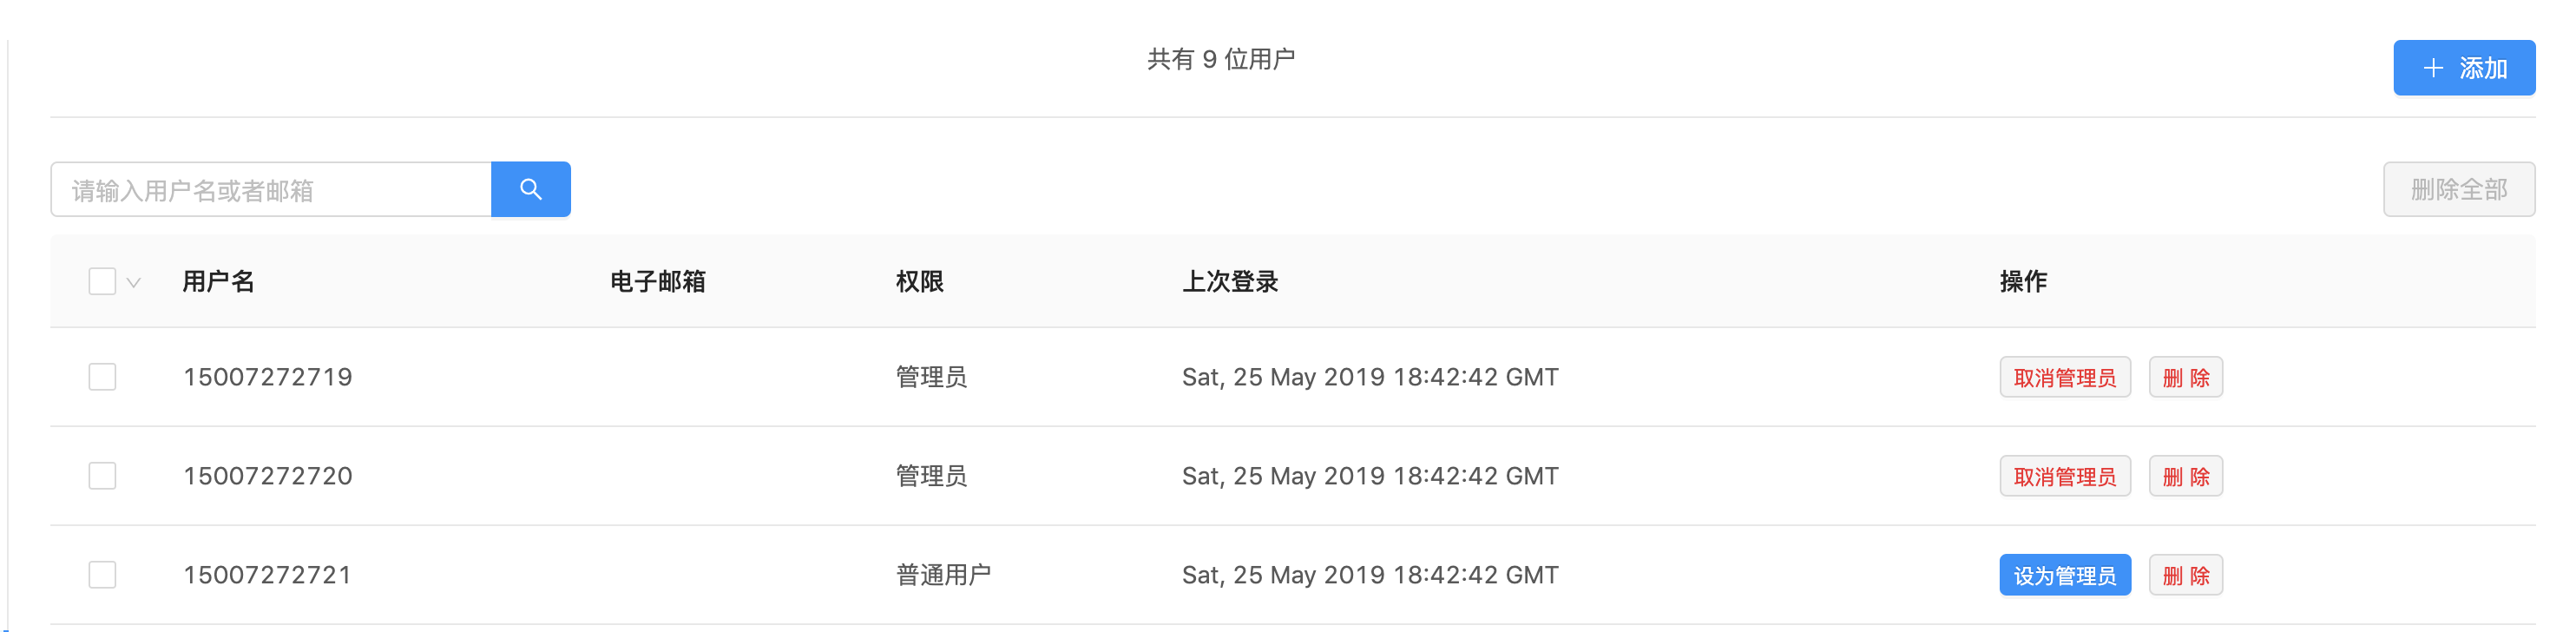
\includegraphics[width=1.0\linewidth]{figure/admin_user}
	\caption{管理用户}
	\label{fig:admin_user}
\end{figure}

\begin{figure}[thbp!]
	\centering
	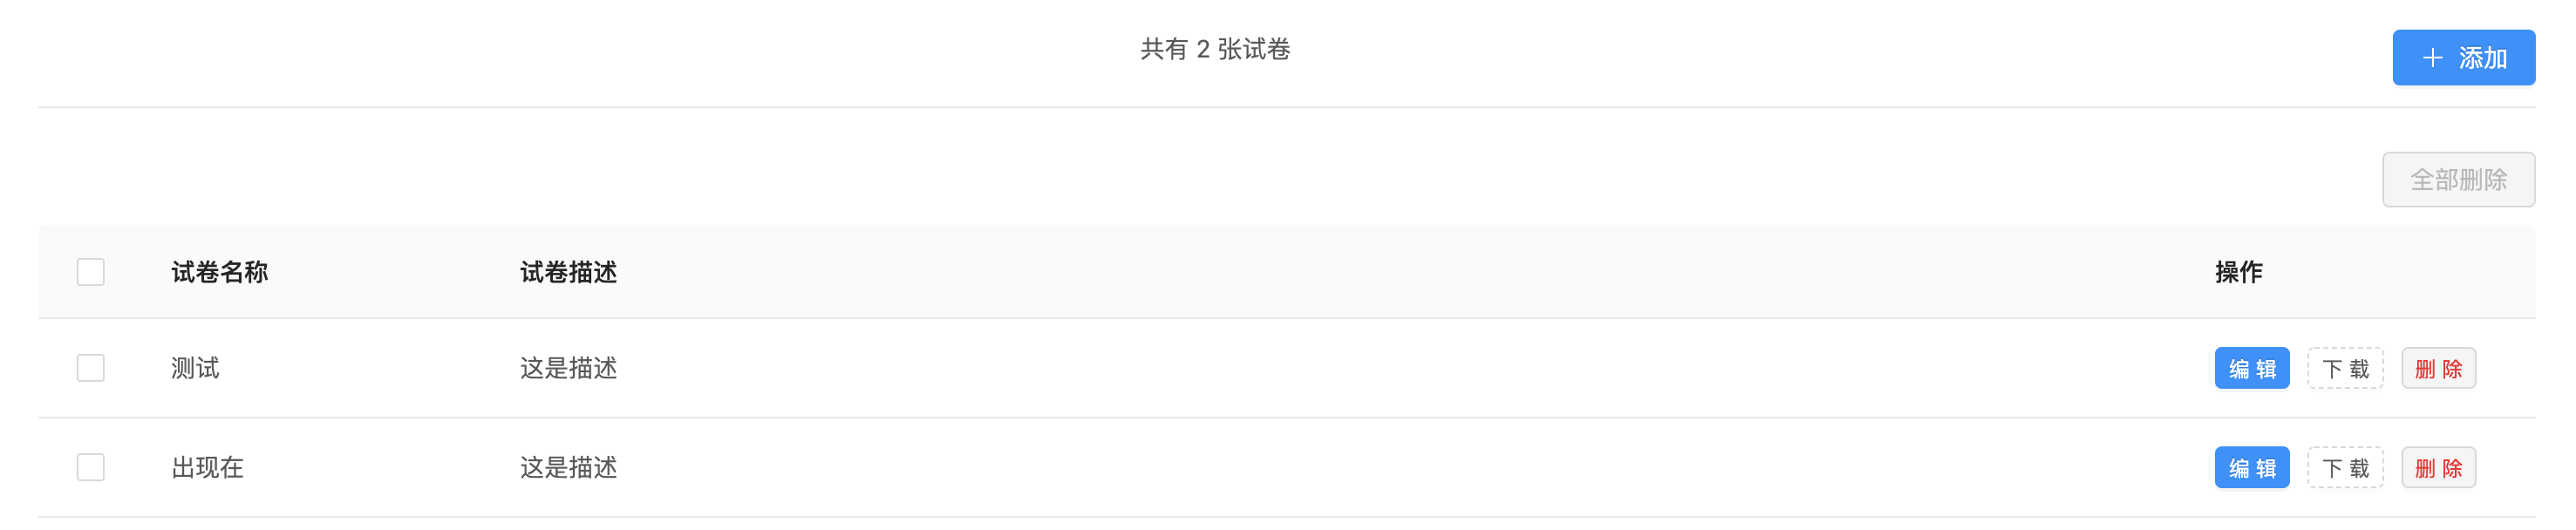
\includegraphics[width=1.0\linewidth]{figure/admin_paper}
	\caption{筛选成绩}
	\label{fig:admin_paper}
\end{figure}

\subsection{评测中心}

\begin{figure}[thbp!]
	\centering
	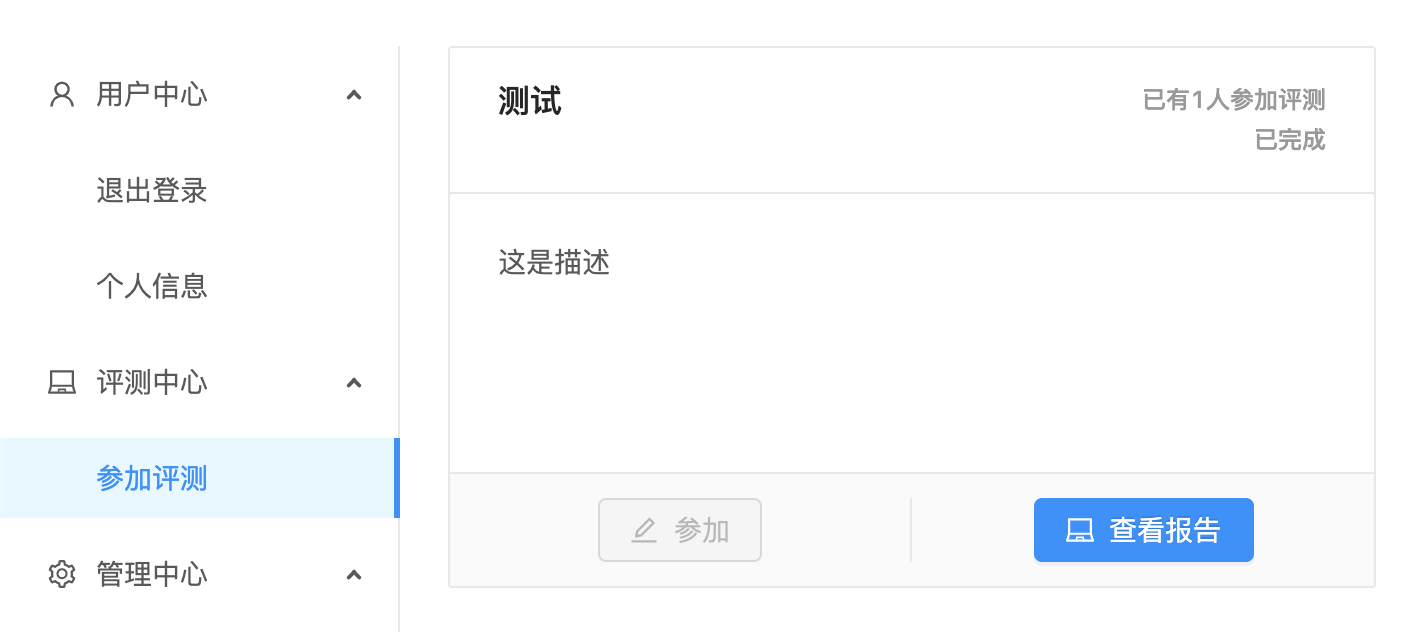
\includegraphics[width=1.0\linewidth]{figure/test}
	\caption{评测中心}
	\label{fig:test}
\end{figure}

\begin{figure}[thbp!]
	\centering
	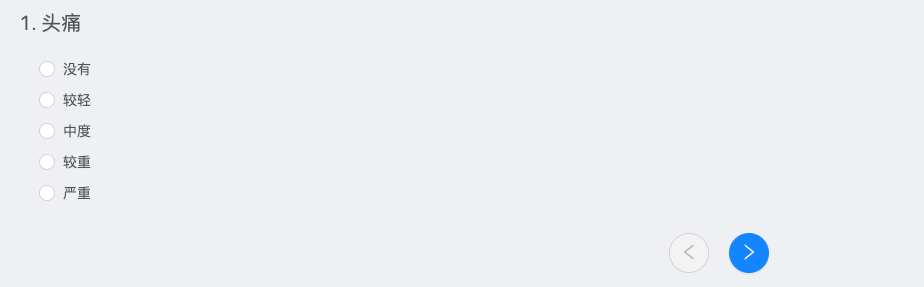
\includegraphics[width=1.0\linewidth]{figure/test_main}
	\caption{评测}
	\label{fig:test_main}
\end{figure}

\begin{figure}[thbp!]
	\centering
	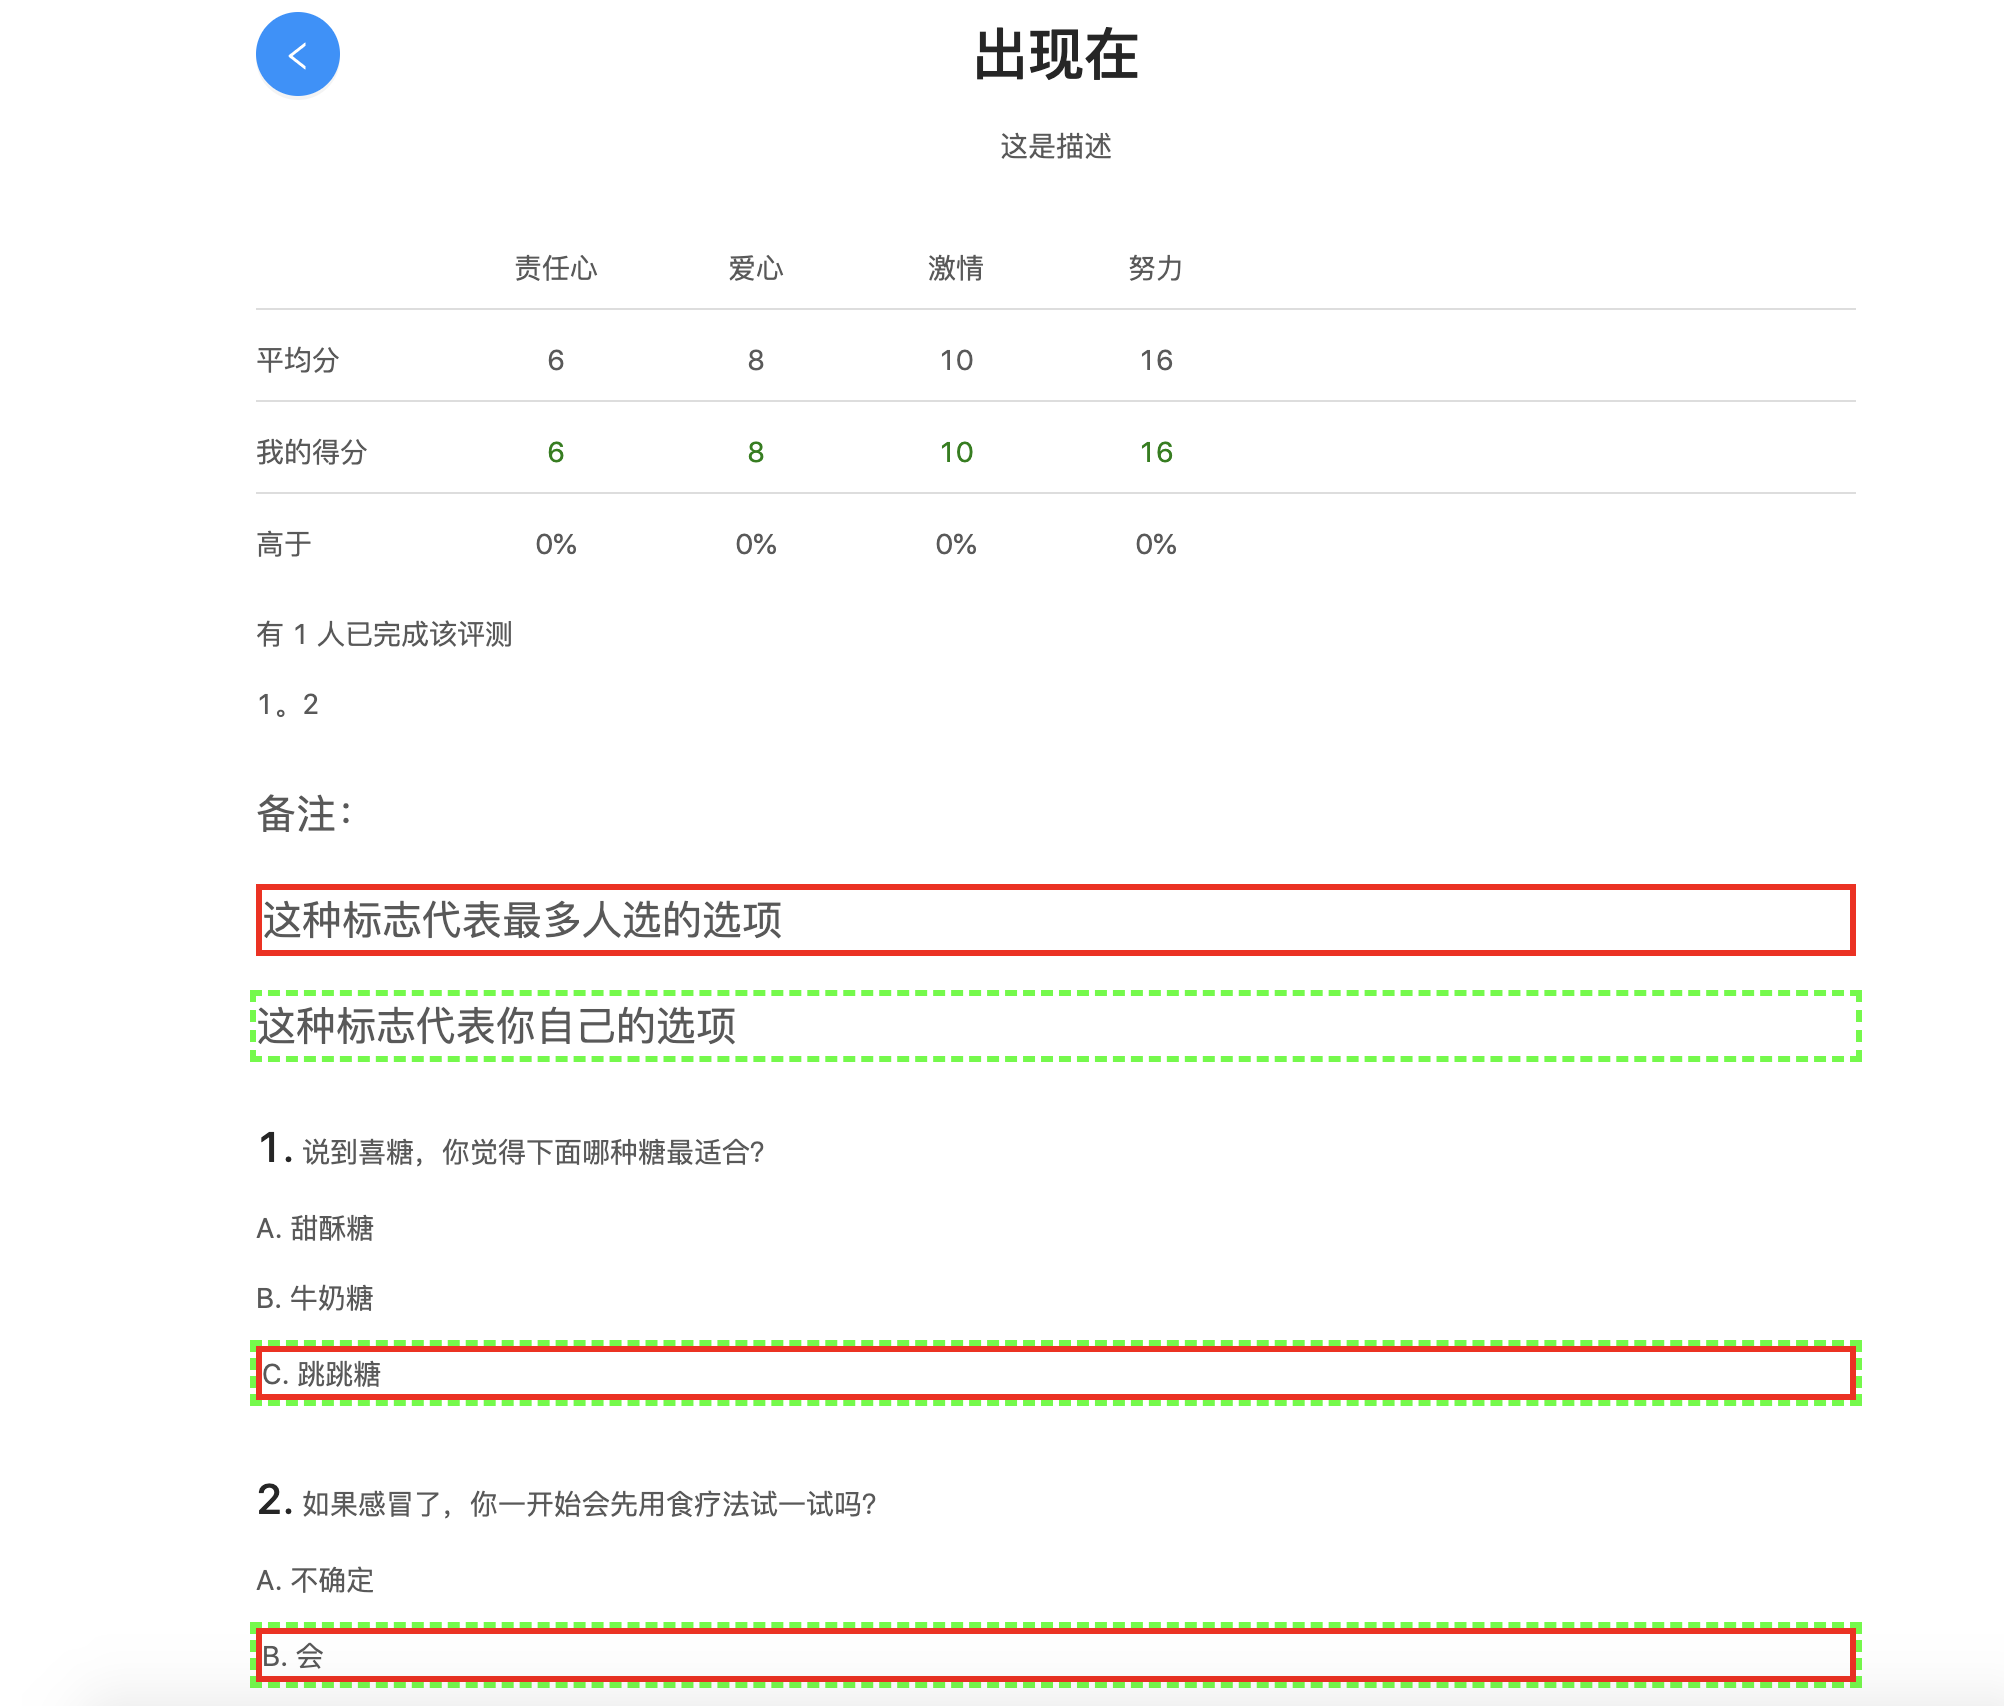
\includegraphics[width=1.0\linewidth]{figure/result_main}
	\caption{评测结果}
	\label{fig:result_main}
\end{figure}